\documentclass[submit]{harvardml}

% You don't need to change these.
\course{CS181-S18}
\assignment{Assignment \#3}
\duedate{11:59pm March 23, 2018}

\usepackage[OT1]{fontenc}
\usepackage[colorlinks,citecolor=blue,urlcolor=blue]{hyperref}
\usepackage[pdftex]{graphicx}
\usepackage{subfig}
\usepackage{fullpage}
\usepackage{amsmath}
\usepackage{amssymb}
\usepackage{color}
\usepackage{todonotes}
\usepackage{listings}
\usepackage{common}
\usepackage{bm}
\usepackage{float}

\usepackage[mmddyyyy,hhmmss]{datetime}

\definecolor{verbgray}{gray}{0.9}
\definecolor{answergreen}{rgb}{0.09,0.42,0.31}

\newenvironment{answer}{%
    \color{answergreen}\bf}
  {%
  }

\lstnewenvironment{csv}{%
  \lstset{backgroundcolor=\color{verbgray},
  frame=single,
  framerule=0pt,
  basicstyle=\ttfamily,
  columns=fullflexible}}{}

%\newcommand{\bX}{\mathbf{X}} %%%% WARNING: may cause unexpected behavior
%\newcommand{\by}{\mathbf{y}} %%%% WARNING: may cause unexpected behavior

%\newcommand{\bw}{\mathbf{w}} %%%% WARNING: may cause unexpected behavior
%\newcommand{\bS}{\mathbf{S}} %%%% WARNING: may cause unexpected behavior

%\newcommand{\mBI}{\mathbb{I}_{ik}} %%%% WARNING: may cause unexpected behavior
%%\newcommand{\bpi}{\mathbf{\pi}} %%%% Already built into latex 

%%\newcommand{\bmu}{\mathbf{\mu}} %%%% Already built into latex 
%\newcommand{\bvar}{\mathbf{\sigma}^2} %%%% WARNING: may cause unexpected behavior
%\newcommand{\bSig}{\mathbf{\Sigma}} %%%% WARNING: may cause unexpected behavior
%\newcommand{\lsum}{\mathlarger{\sum}} %%%% WARNING: may cause unexpected behavior

\begin{document}
\begin{center}
{\Large Homework 3: Max-Margin and SVM}\\
\end{center}
\subsection*{Introduction}

This homework assignment will have you work with max-margin methods
and SVM classification. The aim of the assignment is (1) to further
develop your geometrical intuition behind margin-based classification
and decision boundaries, (2) to have you implement a basic Kernel-based
classifier and get some experience in implementing a model/algorithm 
from an academic paper in the field, and (3) to have you reflect on the
ethics lecture and to address the scenario discussed in class
in more depth by considering the labor market dynamically.

There is a mathematical component and a programming component to this
homework.  Please submit your PDF and Python files to Canvas, and push
all of your work to your GitHub repository. If a question requires you
to make any plots, like Problem 3, please include those in the
writeup.

\newpage
%%%%%%%%%%%%%%%%%%%%%%%%%%%%%%%%%%%%%%%%%%%%%
% Problem 1
%%%%%%%%%%%%%%%%%%%%%%%%%%%%%%%%%%%%%%%%%%%%%
\begin{problem}[Fitting an SVM by hand, 7pts]
  For this problem you will solve an SVM without the help of a
  computer, relying instead on principled rules and properties of
  these classifiers.

Consider a dataset with the following 7 data points each with $x \in \reals$ : \[\{(x_i, y_i)\}_i =\{(-3
, +1 ), (-2 , +1 ) , (-1,  -1 ), (0, -1), ( 1 , -1 ), ( 2 , +1 ), ( 3 , +1 )\}\] Consider
mapping these points to $2$ dimensions using the feature vector $\bphi(x) =  (x, x^2)$. The hard margin classifier training problem is:
%
\begin{align}
  &\min_{\mathbf{w}, w_0} \|\mathbf{w}\|_2^2 \label{eq:dcp} \\
  \quad \text{s.t.} \quad & y_i(\mathbf{w}^\top \bphi(x_i) + w_0) \geq 1,~\forall i \in \{1,\ldots, n\}\notag
\end{align}

The exercise has been broken down into a series of questions, each
providing a part of the solution. Make sure to follow the logical structure of
the exercise when composing your answer and to justify each step.

\begin{enumerate}
\item Plot the training data in $\reals^2$ and draw the decision boundary
of the max margin classifer.
%
\item  What is the value of the margin achieved by the optimal
decision boundary? 
%
\item What is a vector that is orthogonal to the decision boundary?

%
\item Considering discriminant $h(\bphi(x);\boldw,w_0)=\boldw^\top\bphi(x) +w_0$, 
give an expression for {\em all possible} $(\boldw,w_0)$ that define
the optimal decision boundary. Justify your answer.

  \item Consider now the training problem~\eqref{eq:dcp}. Using
your answers so far, what particular solution
to $\boldw$ will be optimal for this optimization
problem?

  \item Now solve for
the corresponding value of $w_0$, using your general expression 
from part~(4.) for the optimal decision boundary.
Write down the discriminant
function $h(\bphi(x);\boldw,w_0)$.


\item What are the support vectors of the classifier?  Confirm that the solution in part~(6.) makes
    the constraints in~\eqref{eq:dcp} binding for support vectors.

\end{enumerate}

\end{problem}
\subsection*{Solution 1}
    \begin{enumerate}
        \item Plot the training data in $\reals^2$ and draw the decision boundary of the max margin classifer.

            \begin{figure}[H]
                \centering
                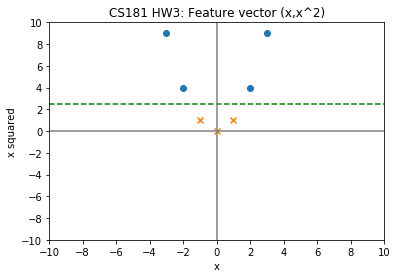
\includegraphics[width=0.5\textwidth]{problem1.png}
                \caption{}
                \label{Problem 1, part 1.}
            \end{figure}

        
        \item  What is the value of the margin achieved by the optimal decision boundary? 

\begin{answer}
            Minimum distance from point to boundary is 1.5 % (4-1)/2 
\end{answer}
            
        \item What is a vector that is orthogonal to the decision boundary?

            \begin{answer}
                Any vertical vector is. e.g. (0,10). Abstractly, $\boldw$.
            \end{answer}

        \item Considering discriminant $h(\bphi(x);\boldw,w_0)=\boldw^\top\bphi(x) +w_0$, give an
            expression for {\em all possible} $(\boldw,w_0)$ that define the optimal decision boundary.
            Justify your answer.

            \begin{answer}
 
                Our decision boundary by visual inspection is at $x^2 = 2.5$.
                Our decision boundary is $h = \boldw^\top\bphi(x) +w_0$.
                \begin{align*}
                    \boldw^T \begin{bmatrix} x \\ x^2 \end{bmatrix} + w_0 = 0 \\ 
                    \begin{bmatrix} w_1 & w_2 \end{bmatrix}  
                    \begin{bmatrix} x \\x^2 \end{bmatrix} + w_0= 0 \\
                    w_1x + w_2x^2 + w_0 = 0 \\
                    \text{Our decision boundary by visual inspection is $x^2 = 2.5$.}\\
                    \text{Thus we get that} \\
                    w_1x=0 \\
                    x^2 = - \frac{w_0}{w_2} = 2.5\\
                    \text{Rewriting in terms of $w_2$ we get}\\
                    w_0  = - 2.5 * w_2  \\
                    \text{For final answer} \\
                    w_2x^2 - 2.5 \cdot  w_2 = 0 \\
                    w_0 = -2.5 \cdot w_2 \\
                    \text{Equivalently in matrix form, } \\
                    \begin{bmatrix} 0 & w_2 \end{bmatrix}  
                    \begin{bmatrix} x \\ x^2 \end{bmatrix} -2.5 \cdot w_2 = 0 %%%should this be > 1????
                \end{align*}

            \end{answer}

        \item Consider now the training problem~\eqref{eq:dcp}. Using your answers so far, what
            particular solution to $\boldw$ will be optimal for this optimization problem?
\begin{answer}
             \begin{align*}
                 &\min_{\mathbf{w}, w_0} \|\mathbf{w}\|_2^2 \label{eq:dcp} \\
                 \quad \text{s.t.} \quad & y_i(\mathbf{w}^\top \bphi(x_i) + w_0) \geq 1,~\forall i \in \{1,\ldots, n\}
             \end{align*}
             If we plug in one of the points we can see by visual inspection is a support vector
             (-2,1) and taking the optimal
             solution to be where the above expression $ y_i(\mathbf{w}^\top \bphi(x_i) + w_0) =
             1,~\forall i  $, we get that 

             \begin{align*}
                 1 (w_2(-2)^2 - w_2 \frac{5}{2} = 1 \\
                 4 w_2 - 2.5w_2 =1  \\
                 w_2 = \frac{1}{1.5} = \frac{2}{3} \\
             \end{align*}

    \end{answer}

        \item Now solve for the corresponding value of $w_0$, using your general expression from
            part~(4.) for the optimal decision boundary.  Write down the discriminant function
            $h(\bphi(x);\boldw,w_0)$.

            \begin{answer}
                Given that $w_2 = 2.5$, we get that
                \begin{align*}
                    w_2 &= \frac{2}{3} \\
                    w_0 &= -\frac{5}{3} \\
                    h(x) &= (2/3) x^2 - 5/3
                \end{align*}
            \end{answer}

        \item What are the support vectors of the classifier?  Confirm that the solution in part~(6.)
            makes the constraints in~\eqref{eq:dcp} binding for support vectors.
\begin{answer} 
    
    %According to reference.com, ``A binding constraint is a constraint used in linear
    %programming equations whose value satisfies the optimal solution; any changes in its value
    %changes the optimal solution."


    Plugging in the points directly, we get that 

    \begin{align*}
        h(-3) &= (2/3)\cdot 9 - (5/3) =  13/3 \\
        h(-2) &= (8/3) - (5/3) =  1 \\
        h(-1) &= (2/3) - (5/3) =  -1 \\
        h(0) &= (0) - (5/3) =  -5/3 \\
        h(1) &= (2/3) - (5/3) =  -1 \\
        h(2) &= (8/3) - (5/3) =  1 \\
        h(3) &= (18/3) - (5/3) =  13/3 \\
    \end{align*}

    Our support vectors are (-2,1), (1,-1),  (-1,1), and (2,1) in terms of (x,y). These points
    optimize our constraint that h(x) $\geq$ 1.

    %We can see that if we moved any of the support vectors, they would either stop being support
    %vectors or our margin would decrease or increase.

    %e.g. if we added a point (1.75, 1), we would need to resolve. The new w's we get would show that
    %for the original four support vectors, the constraint $>$ holds, but it is this new point that
    %constrains the minimum, as that point defines where the constraint $y_i(\boldw^T \phi(x_i) +
    %w_0) = 1.$ 


\end{answer}

    \end{enumerate}
\newpage
%%%%%%%%%%%%%%%%%%%%%%%%%%%%%%%%%%%%%%%%%%%%%
% Problem 2
%%%%%%%%%%%%%%%%%%%%%%%%%%%%%%%%%%%%%%%%%%%%%

\begin{problem}[Scaling up your SVM solver, 10pts (+opportunity for extra credit)]


  For this problem you will build a simple SVM classifier for a binary
  classification problem. We have provided you two files for
  experimentation: training \textit{data.csv} and validation
  \textit{val.csv}.
\begin{itemize}
\item First read the paper at
  \url{http://www.jmlr.org/papers/volume6/bordes05a/bordes05a.pdf} and
  implement the Kernel Perceptron algorithm and the Budget Kernel
  Perceptron algorithm. Aim to make the optimization as fast as possible.
  Implement this algorithm in \textit{problem2.py}.

  [Hint: For this problem, efficiency will be an issue. Instead of directly
implementing this algorithm using numpy matrices, you should utilize
Python dictionaries to represent sparse matrices. This will be necessary 
to have the algorithm run in a reasonable amount of time.   
]
\item Next experiment with the hyperparameters for each of these
  models. Try seeing if you can identify some patterns by changing
  $\beta$, $N$ (the maximum number of support vectors), or the number
  of random training samples taken during the Randomized Search
  procedure (Section 4.3).  Note the training time, training and
  validation accuracy, and number of support vectors for various
  setups.
\item Lastly, compare the classification to the naive SVM imported from
scikit-learn by reporting accuracy on the provided validation
data. {\em For extra credit, implement the SMO algorithm and implement
  the LASVM process and do the same as above.}\footnote{Extra credit
  only makes a difference to your grade at the end of the semester if
  you are on a grade boundary.}

\end{itemize}


We are intentionally leaving this problem open-ended to allow for
experimentation, and so we will be looking for your thought process
and not a particular graph.  Visualizations should be generated 
using the provided code. You can use the trivial
$K(\boldx,\boldx') = \boldx^\top \boldx'$ kernel for this problem,
though you are welcome to experiment with more interesting kernels
too.


In addition, provide answers the following reading questions
{\bf in one or two sentences for each}.
%
\begin{enumerate}
\item In one short sentence, state the main purpose of the paper.
\item Describe each of the parameters in Eq.~1 in the paper
\item State, informally, one guarantee about the Kernel perceptron algorithm described in the
  paper. 
\item What is the main way the budget kernel perceptron algorithm tries to
  improve on the perceptron algorithm?
\item ({\em if you did the extra credit}) In simple words, what is the theoretical guarantee of LASVM algorithm? How
  does it compare to its practical performance?
\end{enumerate}


\end{problem}

\subsection*{Solution 2}
\begin{enumerate}
\item Next experiment with the hyperparameters for each of these
  models. Try seeing if you can identify some patterns by changing
  $\beta$, $N$ (the maximum number of support vectors), or the number
  of random training samples taken during the Randomized Search
  procedure (Section 4.3).  Note the training time, training and
  validation accuracy, and number of support vectors for various
  setups.
  \begin{answer}

            \begin{figure}[H]
                \centering
                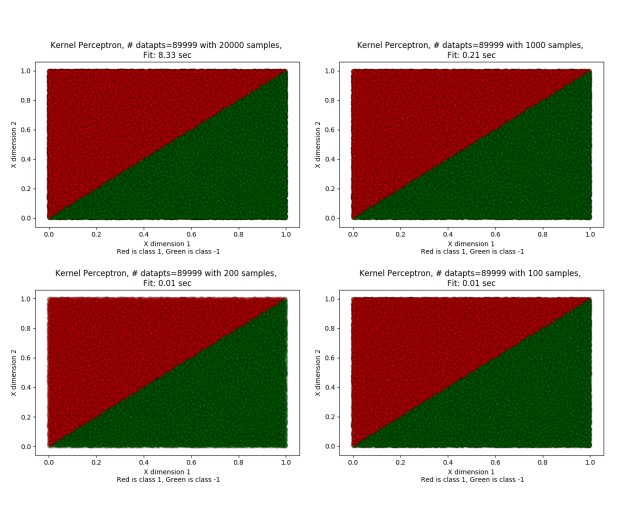
\includegraphics[width=0.7\textwidth]{kernel.png}
                \caption{It seems that the Kernel Perceptrons does very well even just sampling 100
                points out of the 90k datapoints.}
                \label{Problem 1, part 1.}
            \end{figure}

            \begin{figure}[H]
                \centering
                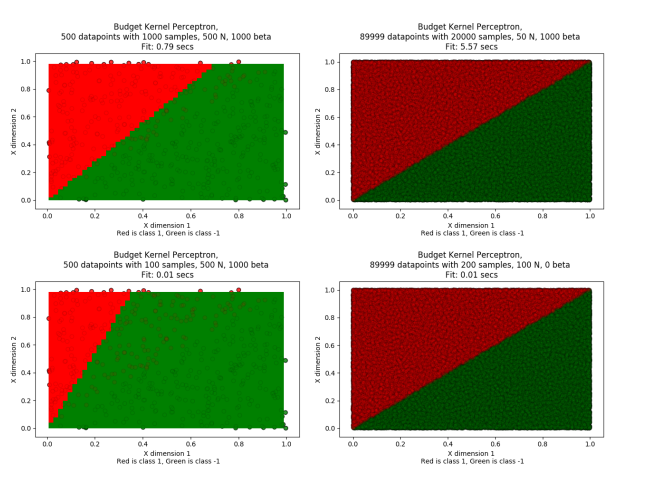
\includegraphics[width=0.7\textwidth]{budget.png}
                \caption{The budget perceptron, we can see, takes 5.6 seconds instead of 8.3 seconds
                on sampling 20k points (out of 90k), and achieves similar accuracy with only 50
            support vectors. Additionally it appears to match the kernel perceptron in performance. Please ignore the graphs on the left (which were drawn from a tiny
        subset of the 90k training data).}
                \label{Problem 1, part 1.}
            \end{figure}




            \begin{figure}[H]
                \centering
                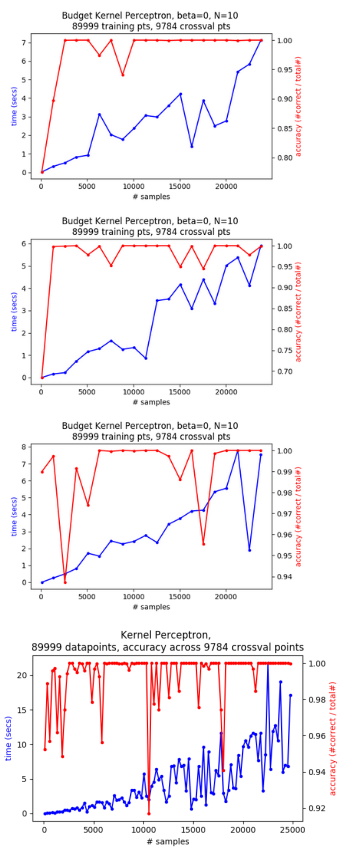
\includegraphics[width=0.5\textwidth]{samplesvstime.png}
                \caption{Samples vs Time. We can see that (a) the SVM is very sensitive to the
                initial randomly selected points (the three top graphs are all different) and (b)
            the budget perceptron does improve on the time required to train -- at 15000 samples, it
        takes 3 seconds instead of 5 seconds. The data is very noisy, perhaps in part due to being
    run inside a virtual machine while other processes are running, but in general we see a trend
toward higher accuracy (against the cross validation set) as number of samples increases. In fact it
seems like we only need 2500 or so data points, not 20k, out of the original set of 90k, in order to
potentially have high accuracy.}
                \label{Problem 1, part 1.}
            \end{figure}

            \begin{figure}[H]
                \centering
                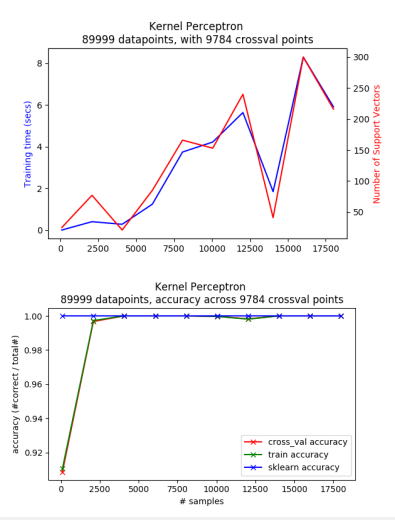
\includegraphics[width=0.5\textwidth]{kernel_numsamples.png}
                \caption{Kernel perceptron, run using a varying number of randomly drawn samples. We
                can see again that around 2500 samples we already have high accuracy. The number of
                support vectors and time to train both increase, as expected. The sklearn
            SVM (with linear kernel) again seems to have perfect accuracy, I suspect there is a bug in my code.}
                \label{Problem 1, part 1.}
            \end{figure}

            \begin{figure}[H]
                \centering
                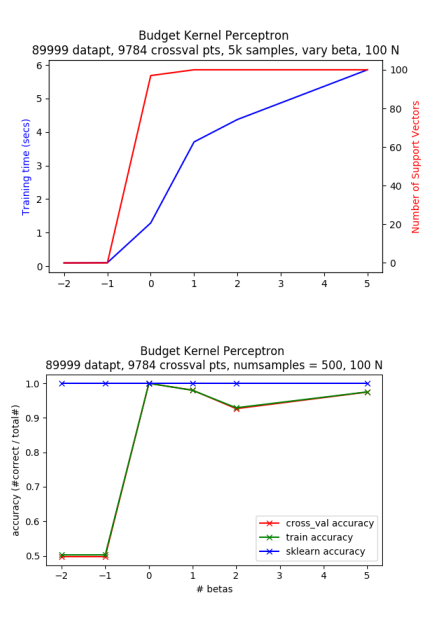
\includegraphics[width=0.5\textwidth]{budget_vs_beta.png}
                \caption{Budget version, vs changes in beta. We see that we want beta to be at least
                zero, or else all examples are misclassified. Zero also appears to be sufficient for
            accuracy purposes. Not that zero does mean that we have fewer than our max number of
        support vectors, vs when beta is 1 or higher.}
                \label{Problem 1, part 1.}
            \end{figure}

            \begin{figure}[H]
                \centering
                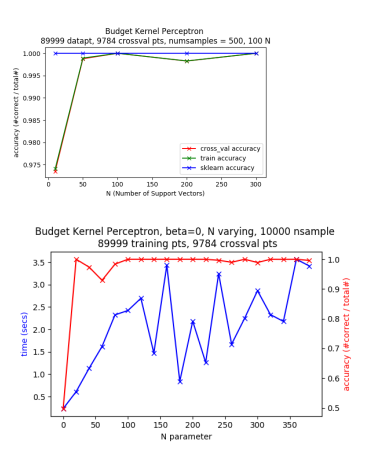
\includegraphics[width=0.6\textwidth]{budget_N.png}
                \caption{Budget version, vs changes in N (number of support vectors). At 50 or so
                support vectors we already have very good accuracy. As number of support vectors
            allowed goes up, the time to train goes up as well. }
                \label{Problem 1, part 1.}
            \end{figure}


            \begin{figure}[H]
                \centering
                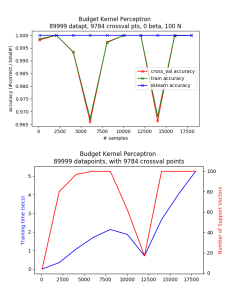
\includegraphics[width=0.4\textwidth]{budget_vs_numsamp.png}
                \caption{Budget version, vs number of randomly drawn training samples, There 
                is a stray datapoint due to a copy paste error, but overall we can see that again at 2500 samples we
            have good accuracy, and 100 support vectors is sufficient. The training time remains
        significantly below that of the kernel. }
                \label{Problem 1, part 1.}
            \end{figure}
            In conclusion: beta = 0, N = 100, and number of samples = 5000 appear to be good
            (somewhat optimal) choices. The budget version performs just as well with less training
            time. We note that the SVM appears to perform very well on the
            cross validated data when fitted against the test data -- this may be to a bug in the
            hand-written accuracy calculation scoring function.


  \end{answer}
\item Lastly, compare the classification to the naive SVM imported from
scikit-learn by reporting accuracy on the provided validation
data. {\em For extra credit, implement the SMO algorithm and implement
  the LASVM process and do the same as above.}\footnote{Extra credit
  only makes a difference to your grade at the end of the semester if
  you are on a grade boundary.}


\item In one short sentence, state the main purpose of the paper.

    \begin{answer}
        This paper describes ways to improve the computational efficiency of SVM classifiers when
        dealing with large and potentially noisy datasets, including random sampling, removing
        support vectors and selectively picking training samples.
    \end{answer}
\item Describe each of the parameters in Eq.~1 in the paper

    \begin{answer}
        $$
        \hat{y}(x) = w'\bPhi(x) + b
        $$

        $\hat{y}$ is our estimate of the true class, either -1 or 1.

        $\bPhi(x)$ is our feature function, which transforms our data into a space where they are
        (hopefully) linearly separable. It is often hand-chosen, for instance in the problem set
        problem above, we were given $f(x) = (x, x^2)$.

        $w$ and $b$ are parameters we find by learning on a set of training examples for which we
        have the true class (or think we do).

    \end{answer}

\item State, informally, one guarantee about the Kernel perceptron algorithm described in the
  paper. 

    \begin{answer}
        If a solution exists, the kernel perceptron will converge to it after a finite number of
        iterations.
    \end{answer}

\item What is the main way the budget kernel perceptron algorithm tries to
  improve on the perceptron algorithm?

    \begin{answer}
        The budget versions maintains a limit on the number of support vectors, discarding the ones
        that are the furthest away from the margin as needed. This allows it to maintain sparsity
        (of support vectors, v.s total number of training examples) and to run on noisy data in a
        computationally efficient manner.
    \end{answer}
\item ({\em if you did the extra credit}) In simple words, what is the theoretical guarantee of LASVM algorithm? How does it compare to its practical performance?

    \begin{answer}
    LASVM will exactly reach the SVM solution after a sufficient number of epochs. Additionally, the
    authors found that after just one epoch, the LASVM error rate closely approached LIBSVM
    accuracy.
    \end{answer}

\end{enumerate}




\newpage
%%%%%%%%%%%%%%%%%%%%%%%%%%%%%%%%%%%%%%%%%%%%%
% Problem 3
%%%%%%%%%%%%%%%%%%%%%%%%%%%%%%%%%%%%%%%%%%%%%
\begin{problem}[Ethics Assignment, 10pts]
Recall our class activity:
\begin{quote}
Hiring at Abercrombie and Fitch. Abercrombie and Fitch have hired a new computer science team to design an algorithm to predict the success of various job applicants to sales positions at Abercrombie and Fitch. As you go through the data and design the algorithm, you notice that African-American sales representatives have significantly fewer average sales than white sales representatives. The algorithm's output recommends hiring far fewer African-Americans than white applicants, when the percentage of applications from people of various races are adjusted for.   
\end{quote}

In class, we thought about the problem \textit{statically}: given historical data, such as data about sales performance, who should Abercrombie and Fitch hire right now? 

In this follow-up assignment, I want you to think about consumer behavior and firm hiring practice dynamically. Looking at features of the labor market dynamically allows you more, or different, degrees of freedom in your model. For example, in class, you probably took consumer preference about the race of their sales representative as given. What would happen if you allowed consumer preference to vary (say, on the basis of changing racial demographics in the sales force)?  

Here’s the new case:
\begin{quote}
The US Secretary of Labor has heard about your team's success with Abercrombie and Fitch and comes to you with a request. The Department of Labor wants to reduce disparate impact discrimination in hiring. They want you to come up with a model of fair hiring practices in the labor market that will reduce disparate impact while also producing good outcomes for companies. 
\end{quote}
Write two or three paragraphs that address the following:
\begin{itemize}
\item What are the relevant socially good outcomes, for both workers and companies?
\item What are some properties of your algorithm that might produce those socially good results?
\begin{itemize}
\item Think about constraints that you might build in, such as the fairness constraints that we discussed in class, or how you might specify the prediction task that we are asking the machine to optimize. 
\end{itemize}
\item Are there tradeoffs that your algorithm has to balance? [optional] 
\item Are there any features of data collection, algorithm implementation, or the social world that make you wary of using machine learning in this case? [optional]
\end{itemize}

We expect that:
\begin{itemize}
\item You focus on one or two points of discussion for each question. 
\begin{itemize}
\item For example, for question 2, pick a single fairness criterion. 
item Depth over breadth here! 
\end{itemize}
\item You provide reasons in support of your answers (i.e., explain why you chose your answer).
\begin{itemize}
\item For example, for the first question, you might choose the socially good outcome of increased profit for companies, and give reasons why profit is the right social goal.
\end{itemize}
\item You are clear and concise - stick to plain, unadorned language.  
\item You do not do any outside research. 
\item You demonstrate a thoughtful engagement with the questions. 
\end{itemize}


\end{problem}

\subsection*{Solution}
    \begin{answer}

In this assignment, we are asked to evaluate the ethical issues in fair hiring practices within
companies that may use algorithms to predict which employee attributes will result in desired
outcomes. Possible relevant social good outcomes that were discussed in class include profit for the
company and equality in employment opportunities for people of different races. In this essay, I
will focus on the reason why socially good outcomes for the employees are a good fairness criteria.
In addition, I will show that the two "categories" of outcomes are in fact interlinked -- what is
good for employees is good for companies.

Good outcomes for the labor market include reducing unemployment and increasing wages
(relative to living cost), ideally bringing equal outcomes to the table, but if not at least trying
to ensure equal access to opportunities. With job stability and a stable health insurance, people
are able to further themselves and their families in social and economic situations. Good outcomes
for the company include being able to continue to exist and being able to profit and grow the
company, ideally by producing value to society, as well as being able to contribute to the
advancement of society. For instance, we are all beneficiaries of companies competing to provide
smartphones, and the companies make money by exploiting a desire we didn't know we had -- to be
constantly connected.

How are these two interlinked? Focusing specifically on race, we may observe that companies tend to have a specific target audience, and larger companies can in fact target more and more niches within a specific target
audience. Thus we can say that, if we had more employees of different races, we would be able to
expand the target market of the company. This would allow a company increase the
size of the "potentential market".  Concretely, say that previously we had a clothing line that was
generic for all races, but not as desirable to either. Now say that we have a clothing line that flatters
pale skin, and one that flatters brown or black skin. In doing so, we can tailor our clothing lines
more (optimistically, we might give differnt sizes and cuts of clothing depending on average
characterics such as height, or, skeptically, simply charge more for superficial changes). By hiring
employees who are able to help with these decisions and expanding this business, we have not only
improved outcomes for racial outcomes at large in society, but also improved outcomes for the
company. Companies that are able to thrive are also able to provide benefits to their employees,
such as a stable job situation, good health benefits, and other forms of stability.

Thus, the situation is much more complex at the company level than simply "hiring the employees with
features, such as race, that correlate with increased sales". In doing so we may miss out on an
extremely profitable opportunity to expand to new markets. I also value the idea of having
more of a feedback mechanism instead, where the model also depends on -- not a quota per se, but on
a "minimum standards" in terms of equality in several dimensions, perhaps race to start. This can be
thought of more theoretically in terms of feedback -- that below a certain percentage of e.g.
African Americans, it becomes very hard to attract and maintain such employees. Thus, we
can add that in as a constraint.

    \end{answer}
\newpage


\subsection*{Calibration [1pt]}
Approximately how long did this homework take you to complete?

25-40 hrs (as usual depending on if you count reading time)

\subsection*{Name, Email, and Collaborators}

Name: Nao Ouyang

Email: nouyang@g.harvard.edu    

Collaborators:
Eric
Wilson
Sharon
Buse
David

\end{document}

\end{document}
